\documentclass[a4paper, utf8, handout]{beamer}

\usepackage [T1]      {fontenc}
\usepackage [english] {babel}

\usepackage {amsmath, amsfonts}
\usepackage {graphicx}

\usepackage {beamer-tools}

% Customs colors
\definecolor {blue}     {RGB} { 40, 80,120}
\definecolor {red}      {RGB} {120, 40, 80}
\definecolor {green}    {RGB} { 80,120, 40}
\definecolor {darkgray} {RGB} { 30, 30, 30}
\definecolor {litegray} {RGB} {245,245,245}

\setuptheme{
  navigation symbols/none,
  % Margins
  margins = {
    % same as frametitle (hard wired in 'beamerbasedefault.sty' l.146)
    text margin left  = 0.3cm,
    text margin right = 0.3cm,
    % footline (also in 'footline' section, see 'headline' below)
    footline margin        = 0.3cm,
    footline margin top    = 0cm,
    footline margin bottom = 0.1cm},
  % --------------------------------------------------------
  % Colors
  colors = {
    normal text  = {fg=darkgray,  bg=litegray},
    structure    = {fg=blue},
    alerted text = {fg=red},
    example text = {fg=green},
    footline     = {parent=headline}},
  % --------------------------------------------------------
  % Fonts
  fonts = {
    normal text  = {size=\normalsize},
    structure    = {series=\bfseries},
    alerted text = {series=\bfseries},
    footline     = {size=\tiny}},
  % --------------------------------------------------------
  % Headline
  headline = {
    % same as frametitle (hard wired in 'beamerbasedefault.sty' l.146)
    margin        = 0.3cm,
    margin top    = 0.1cm,
    margin bottom = 0cm,
    % style
    color = {fg=gray},
    font  = {parent=footline},
    % content
    left  = \slshape\insertshorttitle,
    right = \insertframenumber/\inserttotalframenumber},
  % --------------------------------------------------------
  % Footline
  footline = {
    % content
    left  = \insertshortdate,
    right =\insertshortauthor},
}


%%%%%%%%%%%%%%%%%%%%%%%%%%%%%%%%%%%%%%%%%%%%%%%%%%%%%%%%%%%%


\setuppresentation{
  title        = {Full Title of the Presentation},
  author       = {Bruce Wayne\quad Clark Kent\\
                  Peter Parker\quad Alan Scott},
  date         = {April 01, 2011},
  short title  = {Short Title},
  short author = {Bruce Wayne},
  short date   = {April, 2011},
  institute    = {Justice League of America},
}


%%%%%%%%%%%%%%%%%%%%%%%%%%%%%%%%%%%%%%%%%%%%%%%%%%%%%%%%%%%%


\begin{document}

\begin{frame}[plain]
  \titlepage
\end{frame}


\section
  {Introduction}

\makeatletter
\begin{frame}
  {Introduction}

  {\switchto{example text}Things in a Bulleted List}

  \textin{alerted text}{Things in a Bulleted List}\pause

  \begin{itemize}
  \item With bullets\pause
  \item That come up\pause
  \item One by one
  \end{itemize}
\end{frame}
\makeatother


\section
  {Main Body}

\begin{frame}
  {Equations}

  Equations are easy
  \begin{itemize}
  \item Just copy/paste equations\pause
  \item From the paper!
    \begin{equation*}
      \textbf{p}^* = \underset{\textbf{p}}{\arg\!\min}~\sum_{\textbf{x}}\left[ I(\textbf{W}(\textbf{x};\textbf{p})) - T(\textbf{x}) \right]^2
    \end{equation*}
  \end{itemize}
\end{frame}


\begin{frame}
  {Pictures}

  \begin{figure}[t]
    \centering
    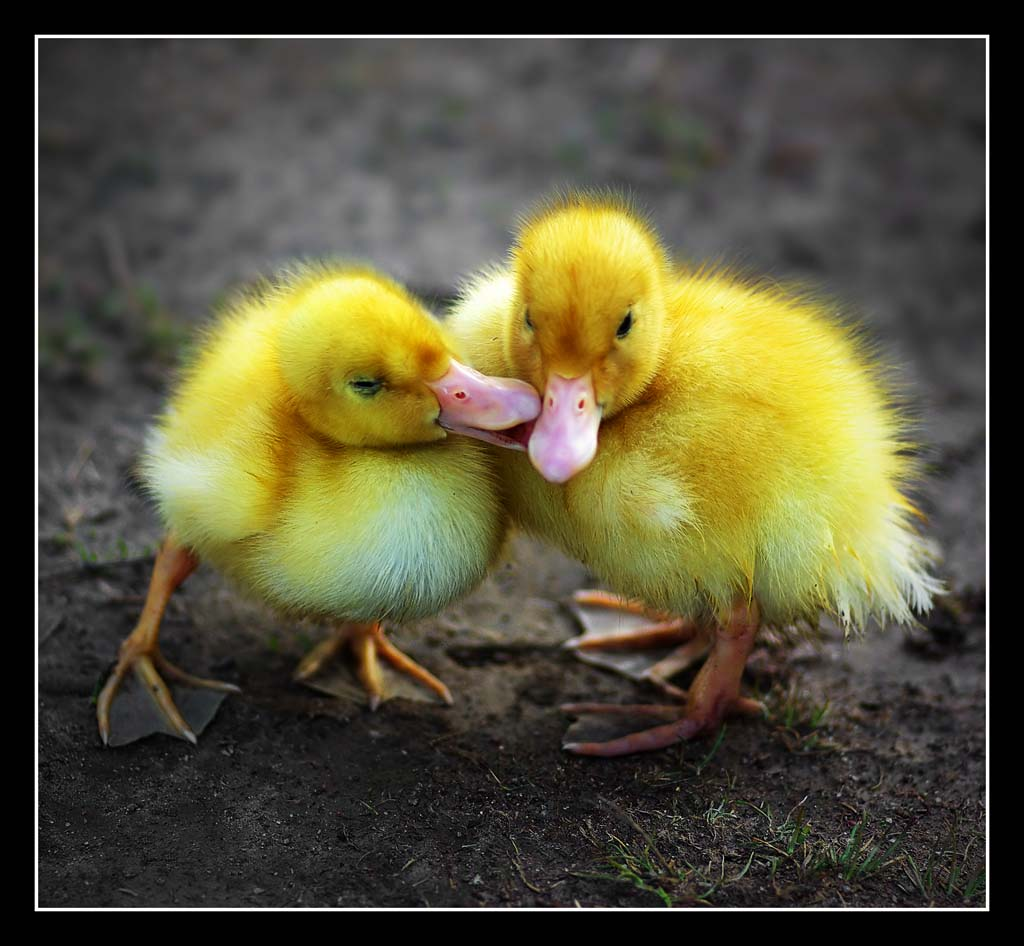
\includegraphics[height=\dimexpr11\textheight/16\relax]{ducks}
    \caption{Kissing ducks}
  \end{figure}
\end{frame}


\begin{frame}
  {A Movie}

  \begin{block}{Some block}
    \begin{itemize}
    \item Movies only seem to work in Adobe Reader
    \item Movie file is not embedded, it must be on the computer
    \end{itemize}
  \end{block}

  \begin{exampleblock}{Some more block}
    Movies only seem to work in Adobe Reader\par
    Movie file is not embedded, it must be on the computer
  \end{exampleblock}

  \begin{alertblock}{Yet another block}
    Some text in here.
    \begin{itemize}
    \item Movies only seem to work in Adobe Reader
    \item Movie file is not embedded, it must be on the computer
    \end{itemize}
  \end{alertblock}

\end{frame}



\section
  {Conclusion}

\begin{frame}
  {Credits}

  \begin{itemize}
  \item Brought to you by Cédric Mauclair
  \item Please let me know about improvements!
  \item inspiration: \url{http://www.shawnlankton.com}... (in code)
  \end{itemize}
\end{frame}


\begin{frame}
  {Questions}

  \nocite{lorem,ipsum}
  \bibliographystyle{plain}
  \bibliography{demo}

\end{frame}

\end{document}
